Fourier volume Registration within the context of a 3D reconstruction procedure requires two frames of 3D data. These two frames may be input as any 3D representation: mesh, volume, point-cloud, SDF or in a compressed format (eg. Octree). However, the input must be converted to a 3D signal or volume representation for phase correlation. Moreover, the size of the volume should be cubic and the data should be scaled to fit. If the two frames are scaled un-evenly then the method must also be registered against scale. This section details some of these issues and more within the context of video sensor input from sensors.  \\
 

\subsubsection{Camera Translation}

To describe camera translation, let's say a camera produces 3D scans of a scene from a particular pose. This may be performed implicitly (in the case of stereo or monocular depth estimation procedures) or explicitly (through the use of such sensors eg. Kinect, Asus Xtion Pro Live) and normalizes them into a 3D volume frames. If the camera captured frame 1, then moves 20 units to the left, then captures frame 2. Visualizing these frames in conjunction with each-other, it would appear the data was shifted to the right by $20$ units ($20\theta$ if the resolution of the 3D volume differs by a scale of $\theta$). If the volumes were to be registered (assuming no error), it would be found that the data from frame 1 to frame 2 had been translated by $T_{frame-1,frame-2} = [20,0,0]^T$, or the translation matrix in equation \ref{eqn:TransRegMatrix}.

\begin{equation} \label{eqn:TransRegMatrix}
\left[
\begin{array}{cccc}
1 & 0 & 0 & 20 \\
0 & 1 & 0 & 0 \\
0 & 0 & 1 & 0 \\
0 & 0 & 0 & 1 \\
\end{array}
\right]
\end{equation}

That is, the data has shifted in the opposite direction. Therefore to register the data, frame 1 may be transformed by the matrix in equation \ref{eqn:TransRegMatrix} to align it with frame 2. Conversely, the camera pose may be updated by adding $T_{frame-1,frame-2} \times -1$ to the camera's location.  \\

Generalizing this, we define a volume $V_1$ captured as the first frame and a second volume $V_2$ which is captured after moving the camera in a particular direction (up, down, left, right, forward or backward) scaled by a magnitude (a vector). The translation from $V_1$ to $V_2$, $(x,y,z)$ can easily be recovered via phase correlation. As described, the camera pose may be updated by $-1 \times (x,y,z) = (-x,-y,-z)$. \\

Here we step into the detail of phase correlation with deeper insight with respect to the superficial introduction from section \ref{Sec:SuperficialPCSection} and with a focus on 3D data and pose estimation. Firstly, we define the correlation measure process. Correlation in the context of signal processing measures signal shape similarity between two signals. \\

In this measure, large correlation values signify a greater similarity in terms of shape, where as a smaller value signifies the signals have very different shapes. Note, large negative values signify the shapes may be similar but mirrored. Following the doctrine of DSP, that all signals, no matter what dimension may be processed similarly with similar operations and measures, this technique can be applied to measure similarities between volumes.  \\

The measure of correlation between $V_1$ and $V_2$ can be found by shifting $V_1$ and $V_2$'s mean values to zero. By doing this, the mean value doesn't affect the correlation measure. For example, if the first frame was captured in low light and the second in a brighter light. The resulting values for frame 2 may look like those from frame 1 in terms of values fluctuating about the mean, however the change in lighting may affect the voxel values by increasing them by a uniform value or scaling them by some scalar. Therefore, by subtracting the mean we place the signals in states where by their shape, rather than their raw values may be compared. The procedure can then be completed by summing the element-wise multiplication of $V_1$ by $V_2$. When $V_1$ has a positive voxel value (a voxel value above the mean) and so does $V_2$'s corresponding voxel in the same position, the multiplication value is positive, and this is summed into the correlation measure. This is the same situation as if both voxel values were negative (both below the mean). On the other hand, if one voxel value was positive and the other were negative, the correlation measure would be rectified accordingly. Equation \ref{eqn:CorrelationEquation} computes this correlation measure. 

\begin{equation} \label{eqn:CorrelationEquation}
\sum_{z=0}^{N}\sum_{y=0}^{N}\sum_{x=0}^{N}(V_1(x,y,z)-avg(V_1)) \times (V_2(x,y,z)-avg(V_2))
\end{equation}

As mentioned, correlation may be used to measure the similarity between two volume's shapes. In the context of registration for 3D reconstruction algorithms, it can be used to measure the accuracy of a registration. Again using $V_1$ as frame 1 and $V_2$ as frame 2, given a supposed transform $T_{est}$ to register $V_1$ to $V_2$. The measure of registration may be defined as $correlate(T_{est}(V_1), V_2)$. The measure may be used to compare two registrations, possibly in order to select the better registration in terms of correlation measure. The two frames may be captured under different lighting conditions and the correlation measure will still be able to be used to select the best transform. \\

Within the framework of measuring camera pose, the cross-correlation algorithm may be used to measure the correlation values for each possible camera movement, and define the camera location as the location with the largest correlation value. This algorithm is shown in listing \ref{algorithm:CrossCorrelationAlgorithm}.

\begin{figure}
\begin{lstlisting}[language=c++,caption=Cross-Correlation based camera location estimation,label=algorithm:CrossCorrelationAlgorithm,mathescape,basicstyle=\ttfamily]
$V_1$ = CaptureFrame();
//shift camera
$V_2$ = CaptureFrame();
$highest-correlation$ = $infty $;
camera-location = $[0,0,0]$;
for($z$ in $[0,N]$){
  for($y$ in $[0,N]$){
    for($x$ in $[0,N]$){
      $V_{temp}$ = translate(V_1, x, y, z);
	  $tempMeasure$ = correlate($V_{temp}$, $V_2$);
	  if($tempMeasure$ > $highest-correlation$){
	    $highest-correlation$ = $tempMeasure$;
		$camera-location$ = $[-x,-y,-z]$;
	  }		
	}
  }
}
\end{lstlisting}
\end{figure}

Cross correlation is typically used in signal processing to compute the best alignment for two signals. In this context it has been used to compute the best camera location change, notice in the algorithm the $camera-location$ variable is set to be the inverse of the translation amount being tested ($[-x,-y,-z]$). Again this is because when the optimal translation value aligning frame 1 to frame 2 is defined as vector $v$, then the camera location change is equivalent to the inverse. The cross-correlation function in this context may be thought of as an exhaustive optimization procedure which optimizes the camera location change (equation \ref{eqn:CrossCorrelationEquation11}) in terms of the correlation function.  \\

\begin{equation} \label{eqn:CrossCorrelationEquation11}
correlate(translate(V_1, x,y,z), V_2)
\end{equation}

The range of camera location vectors to test is dependent on the dimensions of the raw 3D data input. If the data is scaled to fit an $N^3$ space, such as the case where Fourier techniques are implemented, the camera location values along the x, y and z axis would range between 0 and $N$. To compute the optimal camera location change using the phase correlation method would therefore have complexity $N^3$. There are $N^3$ values to test, and the correlate function must be called for each iteration with a complexity also equivalent to $N^3$, $N^3 \times N^3 = N^6$. This is significantly complex, even for smaller volume sizes. Note that the smaller the volume size, the faster the algorithm, however the more quantized the original data is. The more the input data is quantized, the more the camera location change estimate will be restricted in terms of precision. Accuracy will also be affected as quantization introduces unwanted effects of its own. The answer is to use the properties of the Fourier transform to speed up the process.  \\

\begin{figure}[!htb]
\centering
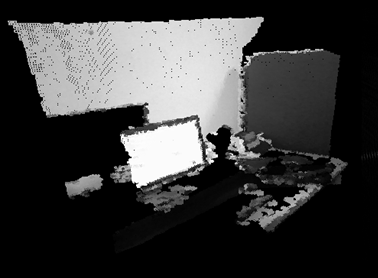
\includegraphics[width=6cm]{images/methodology/FVR/capFrameOriginal}
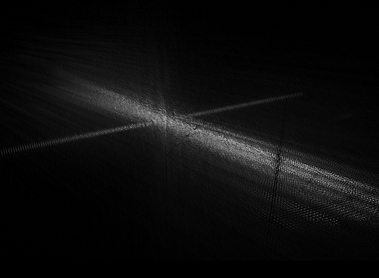
\includegraphics[width=6cm]{images/methodology/FVR/capFrameMagFFT}
\caption{Left: Captured 3D frame, Right: Magnitude values in the frequency domain of the captured 3D frame}
\label{fig:FrequencyDomainExample}
\end{figure}
 
The 3D Fourier transform transforms a volume from the 3D spatial domain into the 3D frequency domain (see figure \ref{fig:FrequencyDomainExample}). The frequency domain is a complex valued volume made up of sinusoids. Each voxel in the frequency domain represents the magnitude, phase and direction of a wave. These properties are important for computing camera pose as shall be discussed upcoming sections. An efficient software implementation of the Fourier transform named the Fast Fourier Transform (FFT) is able to compute the frequency domain given N-dimensional data. \\

Exploiting the properties of the FFT and the frequency domain, cross correlation may be carried out efficiently in order to compute the optimal camera location change between frames. As in the 2D approach, this algorithm is named phase correlation and is a popular approach in 2D image processing to align two images. Applied to two 3D frames captured by sensors (or partially generated via software) it may also be used to register the frames for 3D reconstruction as well as compute the translation part of the camera pose change for SLAM algorithms. The procedure is defined here as a function named $PhaseCorrelation$ (Eq. \ref{eqn:PC_basic}). This function takes two frames (as volumes) as input and returns the best translation alignment between them in terms of maximizing correlation.  \\

\begin{equation} \label{eqn:PC_basic}
T(x, y, z) = PhaseCorrelation(V_x, V_y)
\end{equation}

The $PhaseCorrelation$ consists of 4 steps. In the first step the two captured 3D frames $V_1$ and $V_2$ as transformed into the frequency domain using the Fast Fourier Transform. This computes two new volumes $F_{1_{x,y,z}} = FFT(V_1)$ and $F_{2_{x,y,z}} = FFT(V_2)$. Applying the Fourier Shift Theorem to the context of camera pose estimation, if frames $V_1$ and $V_2$ are separated by some camera translation, then $F_{1_{x,y,z}}$ and $F_{2_{x,y,z}}$ will have phase values shifted relative to each-other. The normalized cross power spectrum (equation \ref{eqn:PHCOR_eq}) of the two complex valued Fourier spaces may then be used to find the camera translation change. The normalized cross power spectrum of $F_{1_{x,y,z}}$ and $F_{2_{x,y,z}}$ is another complex valued volume of the same size. \\

\begin{equation} \label{eqn:PHCOR_eq}
F_{3_{x,y,z}} = \frac{F_{1_{x,y,z}} \circ F_{2_{x,y,z}}^*}{ | F_{1_{x,y,z}} \circ F_{2_{x,y,z}}^* | }
\end{equation}

In equation \ref{eqn:PHCOR_eq}, $\circ$ is an element-wise multiplication and $|x|$ is the magnitude function or absolute value function. The Inverse Fast Fourier Transform ($IFFT$, $FFT^{-1}$) may then be used on the output of the normalized cross power spectrum volume to produce a phase correlation surface. The peak value on the phase correlation surface represents the optimal value of the correlation function applied to the two original real valued 3D frames. Therefore the $PhaseCorrelation$ procedure is equivalent to the cross correlation procedure, but rather than being complexity $N^6$, phase correlation reduces the complexity to approximately $6N^3 \times Log(N)$. \\


Due to the nature of camera capture, if the camera is translated by some vector before the capture of the next frame. Then the first frame contains data which the second frame does not, conversely, the second frame will capture some other data which is not present in the first frame (unless the camera was not moved). The parts of the 3D frames which do not overlap cause noise on the phase correlation surface. This makes it more difficult to decipher the location of the peak. There may be several peaks to choose from, or no clear peak. The nature of computing the Discrete Fourier Transform also affects this. The Discrete Fourier Transform assumes the output Fourier space is an infinitely repeating signal. The cross correlation procedure on the other hand does not assume this, so therefore the phase correlation surface may be affected by this. The solution adopted by many is to filter the volumes prior to transform into the Fourier domain. This can be done using a Hanning window function (equation \ref{eqn:HanningFunction}). This function can be used to filter edge effects on the phase correlation surface. \\

% * (1.0f - cos((2.0f * M_PI * dist) / (hw_dist - 1.0f)))
\begin{equation} \label{eqn:HanningFunction}
Hanning(x) = \frac{1}{2}(1 - cos\left(\frac{2\pi x}{\frac{N}{2} - 1}\right)
\end{equation}

Noise on the phase correlation surface may also be present if other types of transforms are present. In this case, the true camera translation may not be able to be recovered. Therefore, camera pose / rotation must be computed prior to computing the camera translation. Other artefacts which may produce noise on the phase correlation surface include moving objects. If an object is present in one scene and not the other, it will cause some noise to be present in the phase correlation surface, making finding the peak more difficult but not impossible. Alternatively if there is an object whose location is changed between frames, the same thing may happen. The phase correlation procedure should be robust to these artefacts already but filtering approaches may also prove useful in selecting the correct peak which optimizes the translation used to register the 3D camera frames. \\

\subsubsection{Y-Axis Rotation and Scale Registration}

Using the phase correlation procedure along with some spatial transformation functions allows the computation of a single axis of rotation (out of 3) along with the scale difference between two volumes. If $V_1$ and $V_2$ are translated, rotated and scaled versions of the same volume, such that they are related by some translation $(t_x, t_y, t_z)$, y-axis rotation $\theta$, and scale $\varphi$.\\


WARNING: show picture of log-spherical transform\\

Here we describe how to compute the rotation and scale parameters, further action is required to recover translation. The first step, given two volumes $V_1$ and $V_2$ of size $N^3$ is to apply a Hanning windowing function (Eq. \ref{eqn:Hann}). This function assists in filtering the volumes prior to a discrete Fourier transform being applied to them. Since the discrete Fourier transform relies on a continuous signal (volume) and this cannot be used in the calculation, by reducing the signal strength near the volume borders, we can improve the accuracy of the discrete Fourier transform.
\begin{equation} \label{eqn:Hann}
\scriptstyle
HW_{x,y,z} = \frac{1}{2}\left(
1 - cos \left(
\frac{2\pi
\left(
\sqrt{\left(\frac{N}{2}\right)^3} -
\sqrt{
\left(x-\frac{N}{2}\right)^2 + \left(y-\frac{N}{2}\right)^2 + \left(z-\frac{N}{2}\right)^2
}
\right)
}
{2\sqrt{\left(\frac{N}{2}\right)^3} - 1}
\right)
\right)
\end{equation}
The rotation and scale factors can only be recovered if translation information is removed from the two volumes. Therefore we take the magnitude of the FFT of the volumes, $M_1 = |FFT(V_1)|$, $M_2 = |FFT(V_2)|$. Since the magnitude values do not contain phase information they do not, by nature, contain location information of the volume (translation information). The zero-frequency of both $M_1$ and $M_2$ is next shifted to the center of the volume and the log of the result is taken $M'_1 = Log(M_1)$, $M'_2 = Log(M_2)$. Like in phase correlation the log function spreads out the contribution of the frequencies so that high frequencies contribute as much as lower frequencies which have larger magnitudes. A log-spherical transform is then used to turn rotation and scaling into translation for both $M'_1$ and $M'_2$. Eq. \ref{eqn:Log_Spherical} shows the corresponding log-spherical space coordinate $(X_{log-spherical}, Y_{log-spherical}, Z_{log-spherical})$ for a given $(x,y,z)$ euclidean space coordinate.
\begin{equation} \label{eqn:Log_Spherical}
\begin{split}
X_{log-spherical} & = \frac{atan\left(
\left(\frac{x-\frac{N}{2}}{\sqrt{x^2+y^2+z^2}}\right)
\left(\frac{y-\frac{N}{2}}{\sqrt{x^2+y^2+z^2}}\right)^{-1}
\right)N}{360}\\
Y_{log-spherical} & = \frac{acos\left(
\frac{y}{\sqrt{x^2+y^2+z^2}}
\right)N}
{180} \\
Z_{log-spherical} & =\frac{log\left(\sqrt{x^2+y^2+z^2}\right)N}{log\left( \frac{N}{2.56} \right)} \\
\end{split}
\end{equation}
The log-spherical transforms of $M'_1$ and $M'_2$ are then phase correlated to find the shift between them, $(x_{M'},y_{M'},z_{M'}) = PhaseCorrelation(M'_1, M'_2)$. The rotation $\theta$ and scale $\varphi$ factors between $V_1$ and $V_2$ can then be found from the shift parameters using Eq. \ref{eqn:ROTATIONSCALEFROMXM} . 
\begin{equation} \label{eqn:ROTATIONSCALEFROMXM}
\begin{split}
\theta & = \frac{-360x_{M'}}{N}\\
\varphi & = e^{
-\left(
2.56^{-1}N
\right)z_{M'}N^{-1}
}
\end{split}
\end{equation}
Using $\theta$ and $\varphi$, $V_1$ can now be inverse transformed (using $(\frac{N}{2}, \frac{N}{2}, \frac{N}{2})$ as the origin). This aligns $V_1$ and $V_2$ with respect to scale and y-axis rotation. The translation parameters $(t_x, t_y, t_z)$ can then be found using phase correlation as given in Eq. \ref{eqn:FINALTRANS}.
\begin{equation} \label{eqn:FINALTRANS}
(t_x, t_y, t_z) = PhaseCorrelation(scale(rotate(V_1,\theta),\varphi), V_2)
\end{equation}
The complete function to recover translation, rotation and scaling, combining equations \ref{eqn:PHCOR_eq}-\ref{eqn:FINALTRANS} as is denoted in \ref{algorithm:PCSLAM} is \ref{eqn:FULLPC}.
\begin{equation} \label{eqn:FULLPC}
(\theta, \varphi, t_x, t_y, t_z) = PhaseCorrelation_{\theta \varphi t_x t_y t_z}(V_m, V_n)
\end{equation}

